
\section{VANET Simulation Frameworks and Performance Evaluation}
\label{sec:4}

Performance evaluation is a fundamental aspect of
Vehicular Ad Hoc Network (VANET) research because
vehicular communication depends on the interaction
between wireless networking and vehicle mobility.
Unlike conventional wireless networks, VANETs
operate in environments where node positions,
network connectivity, and channel conditions
may change continuously \cite{Hartenstein2008}.

Conducting large-scale real-world experiments
with connected vehicles can be expensive,
time-consuming, and difficult to reproduce.
Simulation-based research therefore provides
an important approach for investigating
communication protocols, network architectures,
and vehicular applications under controlled
conditions \cite{Sommer2011}.

Simulation environments allow researchers
to examine how vehicle density, mobility
patterns, communication technology, routing
protocols, and road topology influence
network performance.

This section reviews established VANET
simulation tools, common evaluation
methodologies, important performance
metrics, and limitations of
simulation-based research.

 This section primarily presents a
literature-based technical review.
In addition, a simplified Python-based
illustrative experiment is included
to demonstrate the relationship between
vehicle density and selected
communication performance metrics.
The experiment does not implement
a complete VANET protocol stack.

\subsection{Simulation-Based VANET Research}
\label{sec:4A}

A realistic vehicular networking study
must consider both transportation
behavior and wireless communication.

The mobility component determines
vehicle positions, speeds, routes,
and interactions with road
infrastructure.

The communication component models
wireless transmissions, message
forwarding, interference, and
protocol behavior.

These components are closely related
because vehicle movement changes
communication topology, while
communication-enabled applications
may influence vehicle behavior
\cite{Sommer2011}.

\subsubsection{Mobility Modeling}

Mobility models describe how vehicles
move through a transportation environment.

A mobility model may represent road
geometry, intersections, traffic lights,
vehicle speeds, and traffic density.

Simplified mobility models can help
isolate individual network
characteristics. However, they may
not capture important transportation
constraints.

Detailed traffic simulation can
provide road layouts and vehicle
movement patterns that more closely
reflect real transportation systems.

\subsubsection{Network Modeling}

Network simulators model communication
behavior between vehicles and
infrastructure nodes.

Depending on the simulator and selected
modules, researchers may investigate
wireless channel access, packet
transmission, routing, interference,
and application traffic.

The validity of a network simulation
depends on the selected propagation
models, protocol implementations,
and configuration parameters.

\subsubsection{Coupled Simulation}

Coupled simulation combines vehicle
mobility modeling with wireless
network simulation.

Vehicle positions and movement data
are exchanged between traffic and
network simulation components.
This allows communication behavior
to reflect changes in vehicle mobility.

Depending on the framework, information
may also flow from network applications
back to the traffic simulation.

Bidirectionally coupled simulation
is especially useful when a networking
application changes vehicle behavior,
which in turn changes the communication
environment \cite{Sommer2011}.

\subsection{Major VANET Simulation Tools}
\label{sec:4B}

Several open-source frameworks support
research on vehicular communication.
These tools differ in their objectives,
simulation models, protocol support,
and integration capabilities.

\subsubsection{Simulation of Urban Mobility}

Simulation of Urban MObility (SUMO)
is an open-source microscopic road
traffic simulator.

It can model individual vehicles,
road networks, intersections,
traffic lights, and vehicle
movement patterns.

SUMO is useful for generating
mobility scenarios that reflect
transportation conditions.

However, SUMO is primarily a
traffic simulator. Detailed wireless
communication experiments require
integration with a suitable
network simulation environment.

\subsubsection{OMNeT++}

OMNeT++ is a discrete-event
simulation framework used for
studying communication systems.

It provides a modular simulation
architecture that can be extended
with network models and protocol
implementations.

In vehicular networking research,
OMNeT++ can be combined with
frameworks that model wireless
communication and vehicle mobility.

Its modular structure makes it
useful for investigating network
protocols under controlled
simulation conditions.

\subsubsection{Veins Framework}

Veins is an open-source vehicular
networking simulation framework
that couples OMNeT++ with SUMO.

The framework enables vehicle
movement and wireless communication
to be investigated within a
coordinated simulation environment.

SUMO provides road traffic behavior,
while OMNeT++ and associated models
represent network communication.

The coupling allows changes in
vehicle position and movement
to influence the wireless
network topology.

This approach supports investigation
of mobility-aware networking and
applications that interact with
traffic behavior \cite{Sommer2011}.

\subsubsection{NS-3}

NS-3 is an open-source discrete-event
network simulator.

It supports research on network
protocols, wireless systems,
and communication performance.

For VANET studies, NS-3 may be
combined with vehicle mobility
data or integrated with external
traffic simulation tools such
as SUMO.

The exact vehicular communication
capabilities depend on the modules,
models, and integrations used
in a particular study.

\subsubsection{Artery and Vanetza}

Artery is an open-source vehicular
networking simulation framework
built around OMNeT++-based simulation.

It supports research related
to cooperative vehicular
communication and European
Intelligent Transportation
Systems technologies.

Vanetza is an open-source
implementation of protocol
components associated with
ETSI Cooperative ITS.

These projects provide useful
resources for investigating
vehicular message processing
and communication protocol behavior.

Their functionality and compatibility
depend on the software versions,
dependencies, and configurations used.

\begin{table*}[t]
\centering
\caption{Comparison of Open-Source Tools Used in VANET Research}
\label{tab:simulation_tools}
\footnotesize
\begin{tabular}{|p{2.0cm}|p{3.1cm}|p{3.6cm}|p{3.6cm}|p{2.9cm}|}
\hline
\textbf{Tool} &
\textbf{Primary Purpose} &
\textbf{Main Strength} &
\textbf{Important Limitation} &
\textbf{Typical Research Use} \\
\hline
SUMO &
Road traffic simulation &
Detailed vehicle movement and road network modeling &
Does not independently provide a complete wireless network simulation &
Mobility and traffic scenarios \\
\hline
OMNeT++ &
Discrete-event simulation framework &
Modular and extensible communication modeling &
Requires appropriate models for specific VANET technologies &
Network and protocol simulation \\
\hline
Veins &
Coupled vehicular network simulation &
Integration of mobility and wireless communication &
Results depend on supported models and simulation configuration &
Mobility-aware VANET studies \\
\hline
NS-3 &
Network simulation &
Detailed network modeling and protocol experimentation &
Vehicular studies may require external mobility integration &
Wireless performance analysis \\
\hline
Artery &
Cooperative vehicular networking simulation &
Support for ETSI-oriented vehicular research &
Requires compatible dependencies and configuration &
Cooperative ITS applications \\
\hline
Vanetza &
Cooperative ITS protocol implementation &
Implementation of ETSI ITS protocol components &
Not a standalone road traffic simulator &
Vehicular protocol research \\
\hline
\end{tabular}
\end{table*}

\subsection{Representative Simulation Scenarios}
\label{sec:4C}

VANET simulation studies investigate
different traffic and communication
environments.

The selected scenario influences
connectivity, channel conditions,
and routing performance.

\subsubsection{Urban Scenarios}

Urban environments typically contain
intersections, traffic signals,
buildings, and complex road networks.

Vehicles may frequently change
direction or experience variable speeds.

Buildings and other obstacles can
affect wireless propagation and
reduce communication reliability.

Urban scenarios are therefore useful
for studying intersection-related
applications, geographic routing,
and communication under obstructed
conditions.

\subsubsection{Highway Scenarios}

Highway environments often involve
higher vehicle speeds and relatively
structured movement patterns.

Relative movement between vehicles
may cause wireless neighbors
to change quickly.

Highway scenarios are useful
for investigating communication
link duration, multihop information
dissemination, and safety warnings.

\subsubsection{Sparse Network Scenarios}

Sparse vehicular networks contain
relatively few participating
communication nodes.

Vehicles may be separated by
distances that prevent continuous
multihop connectivity.

Such scenarios are useful for
evaluating intermittent communication
and delay-tolerant forwarding.

\subsubsection{Dense Network Scenarios}

Dense vehicular networks contain
many nearby communication nodes.

Although higher vehicle density
may improve the availability
of forwarding neighbors,
it can also increase channel
contention and interference.

Dense scenarios are particularly
important for studying congestion
control, broadcast efficiency,
and communication scalability.

\begin{table}[htbp]
\centering
\caption{Representative VANET Evaluation Scenarios}
\label{tab:vanet_scenarios}
\footnotesize
\begin{tabular}{|p{1.4cm}|p{2.3cm}|p{2.7cm}|}
\hline
\textbf{Scenario} &
\textbf{Characteristics} &
\textbf{Main Evaluation Concern} \\
\hline
Urban &
Intersections and obstacles &
Propagation and route selection \\
\hline
Highway &
Higher speeds and changing neighbors &
Link duration and delay \\
\hline
Sparse &
Limited forwarding nodes &
Connectivity and delivery \\
\hline
Dense &
Many simultaneous transmitters &
Congestion and scalability \\
\hline
\end{tabular}
\end{table}

\subsection{Performance Evaluation Metrics}
\label{sec:4D}

Performance metrics provide quantitative
measures for assessing vehicular
communication.

Different metrics describe different
aspects of network behavior.

For meaningful comparisons,
researchers must define metrics
consistently and report relevant
simulation conditions.

\subsubsection{Packet Delivery Ratio}

Packet Delivery Ratio (PDR) represents
the proportion of data packets
successfully received by their
intended destinations.

\begin{equation}
PDR =
\frac{N_{\mathrm{received}}}
{N_{\mathrm{sent}}}
\times 100\%,
\label{eq:pdr}
\end{equation}

where $N_{\mathrm{received}}$
is the number of successfully
received packets and
$N_{\mathrm{sent}}$ is the number
of transmitted data packets
considered in the evaluation.

A higher PDR generally indicates
more successful packet delivery.

However, the interpretation depends
on whether the study uses unicast,
broadcast, or multihop communication.

For broadcast applications,
the number of intended receivers
must be considered explicitly.
Otherwise, PDR values from
different studies may not
be directly comparable.

\subsubsection{Average End-to-End Delay}

End-to-end delay represents the
time between packet transmission
and successful reception.

The average delay is

\begin{equation}
D_{\mathrm{avg}} =
\frac{1}{N}
\sum_{i=1}^{N}
\left(
t_{\mathrm{receive},i}
-
t_{\mathrm{send},i}
\right),
\label{eq:delay}
\end{equation}

where $N$ is the number of
successfully received packets
included in the calculation.

Lower delay is particularly
important for time-sensitive
safety applications.

Average delay alone may not
describe worst-case communication
behavior. Delay distributions
and high-percentile delays
can provide additional information.

\subsubsection{Throughput}

Throughput measures the amount
of successfully delivered data
per unit of time.

\begin{equation}
T =
\frac{B_{\mathrm{received}}}
{\Delta t},
\label{eq:throughput}
\end{equation}

where $B_{\mathrm{received}}$
is the number of successfully
received bits during the
observation interval $\Delta t$.

Throughput may be reported in
bits per second or related units.

Higher throughput can be useful
for data-intensive applications,
but maximizing throughput does
not necessarily minimize delay
or improve safety-message
reliability.

\subsubsection{Packet Loss Ratio}

Packet Loss Ratio (PLR) describes
the proportion of transmitted
packets that are not
successfully received.

\begin{equation}
PLR =
\frac{
N_{\mathrm{sent}}
-
N_{\mathrm{received}}
}{
N_{\mathrm{sent}}
}
\times 100\%,
\label{eq:plr}
\end{equation}

For a consistent unicast packet
accounting model, PDR and PLR
are complementary.

However, special care is required
when evaluating broadcast traffic
or retransmissions.

\subsubsection{Communication Overhead}

Communication overhead describes
the additional resources consumed
by protocol control messages,
signaling, and forwarding operations.

An illustrative normalized
overhead measure can be defined as

\begin{equation}
O =
\frac{
N_{\mathrm{control}}
}{
N_{\mathrm{delivered}}
},
\label{eq:control_overhead}
\end{equation}

where $N_{\mathrm{control}}$
is the number of control packet
transmissions and
$N_{\mathrm{delivered}}$
is the number of successfully
delivered data packets.

A lower control overhead may
indicate more efficient use of
communication resources, although
it should not be interpreted
independently of reliability
and delay.

This definition is consistent
with the illustrative routing
overhead measure discussed
in Section~\ref{sec:3C}.

\subsubsection{Packet Delivery Delay Variation}

Delay variation, often called
jitter, describes changes in
packet delay over time.

One possible measure is the
average absolute difference
between delays of consecutive
received packets:

\begin{equation}
J =
\frac{1}{N-1}
\sum_{i=2}^{N}
|D_i-D_{i-1}|,
\label{eq:jitter}
\end{equation}

where $D_i$ is the end-to-end
delay of packet $i$ and $N>1$.

This is one possible jitter
definition; studies may use
alternative definitions.

Delay variation is relevant
when applications require
consistent communication timing.

\begin{table*}[t]
\centering
\caption{Common VANET Performance Metrics and Their Interpretation}
\label{tab:performance_metrics}
\footnotesize
\begin{tabular}{|p{3.1cm}|p{3.6cm}|p{3.5cm}|p{4.1cm}|}
\hline
\textbf{Metric} &
\textbf{What It Measures} &
\textbf{Typical Desired Direction} &
\textbf{Important Interpretation Issue} \\
\hline
Packet Delivery Ratio &
Successful packet delivery &
Higher &
Depends on traffic and receiver accounting \\
\hline
End-to-End Delay &
Packet delivery time &
Lower &
Mean values may hide delay outliers \\
\hline
Throughput &
Successfully delivered data rate &
Higher for data-oriented services &
Does not independently measure safety reliability \\
\hline
Packet Loss Ratio &
Unsuccessful packet delivery &
Lower &
Must use consistent packet counting \\
\hline
Routing Overhead &
Control traffic relative to delivered data &
Generally lower &
May trade off against reliability \\
\hline
Jitter &
Variation in packet delay &
Generally lower &
Depends on the selected jitter definition \\
\hline
\end{tabular}
\end{table*}

\subsection{Factors Affecting VANET Performance}
\label{sec:4E}

Several factors influence
vehicular communication performance
\cite{Zeadally2012}.

\subsubsection{Vehicle Density}

Vehicle density affects both
connectivity and wireless
channel usage.

At low density, communication
paths may be unavailable because
vehicles are too far apart.

At high density, the increased
number of transmissions may
cause contention and congestion.

Therefore, increasing vehicle
density does not necessarily
improve overall network performance.

\subsubsection{Vehicle Speed and Mobility}

Vehicle speed influences how
quickly communication neighbors
change.

High relative mobility can
reduce the duration of usable
wireless links and increase
route maintenance requirements.

The impact depends on road
layout, movement direction,
and protocol behavior.

\subsubsection{Wireless Propagation}

Wireless propagation conditions
affect the probability of
successful packet reception.

Buildings, vehicles, terrain,
and other obstacles can weaken
or obstruct wireless signals.

The selected propagation model
can therefore strongly influence
simulation results.

\subsubsection{Communication Range}

Communication range influences
the number of potential
neighboring nodes.

A larger effective range may
improve connectivity, but changes
to transmission power and radio
configuration can also affect
interference and channel usage.

Consequently, range-related
parameters should be evaluated
together with reliability
and congestion.

\subsubsection{Routing Protocol}

Routing protocols differ in
route discovery, forwarding,
and maintenance mechanisms.

Their performance depends on
network mobility, traffic density,
and application requirements.

A protocol that performs well
in one scenario may be less
effective under different
conditions.

\subsection{Methodology for Comparing VANET Studies}
\label{sec:4F}

A reliable comparison of published
VANET studies requires careful
consideration of their
experimental settings.

Results from different papers
should not be treated as directly
comparable when they use different
mobility models, communication
technologies, traffic loads,
or metric definitions.

A structured comparison should
consider the following dimensions.

\subsubsection{Scenario Consistency}

Researchers should identify
whether studies use urban,
highway, or other mobility
scenarios.

Road topology, vehicle density,
and speed distributions can
influence network behavior.

\subsubsection{Protocol and Technology Configuration}

Studies may evaluate different
routing protocols, wireless
standards, transmission parameters,
or application traffic patterns.

These settings must be considered
when interpreting reported results.

\subsubsection{Measurement Definitions}

Metrics such as PDR, throughput,
and delay may be calculated
differently across studies.

Comparisons should therefore
examine the underlying definitions
rather than relying only on
metric names.

\subsubsection{Reproducibility}

Reproducible research requires
clear documentation of simulation
tools, software versions,
network parameters, mobility
scenarios, and evaluation
procedures.

Where possible, researchers
should also report repeated
runs and appropriate measures
of result variability.

\begin{table}[htbp]
\centering
\caption{Checklist for Evaluating Published VANET Studies}
\label{tab:study_checklist}
\footnotesize
\begin{tabular}{|p{2.4cm}|p{4.0cm}|}
\hline
\textbf{Dimension} &
\textbf{Information to Examine} \\
\hline
Environment &
Urban, highway, or mixed scenario \\
\hline
Mobility &
Vehicle speed, density, and movement model \\
\hline
Communication &
Wireless technology and channel settings \\
\hline
Protocol &
Routing or dissemination approach \\
\hline
Metrics &
Definitions of PDR, delay, and throughput \\
\hline
Reproducibility &
Software versions, parameters, and repeated runs \\
\hline
\end{tabular}
\end{table}

\subsection{Limitations of Simulation-Based Evaluation}
\label{sec:4G}

Simulation is valuable for
controlled experimentation,
but it has important limitations.

First, simulation results depend
on assumptions about vehicle
behavior and wireless propagation.

Second, simplified models may
not capture all environmental
effects, hardware constraints,
or unexpected road conditions.

Third, the performance of a
protocol under one simulation
configuration does not guarantee
equivalent performance in
a real deployment.

Finally, comparisons between
different studies can be
misleading when experimental
conditions are inconsistent.

These limitations highlight
the importance of transparent
methodologies, careful result
interpretation, and validation
where practical \cite{Sommer2011}.


\subsection{Illustrative Python-Based VANET Simulation}
\label{sec:python_vanet}

To complement the literature-based review,
a simplified Python-based experiment was
implemented to illustrate the relationship
between vehicle density and communication
performance in a VANET environment.

\subsubsection{Simulation Setup}

The experiment was implemented using
Python 3.13 with NumPy and Matplotlib.

Vehicles were randomly positioned along
a one-dimensional road of length 1000 m.
The communication range was fixed at 250 m.

Five vehicle densities were evaluated:
10, 20, 30, 40, and 50 vehicles.
Each vehicle generated 100 packets,
with a randomly selected destination.

Packet delivery was determined using
a simplified probabilistic model based
on communication distance and vehicle count.

Packets sent to destinations beyond
the communication range were considered lost.

The experiment used a fixed random seed
of 42 to support reproducibility.

This model does not implement actual
IEEE 802.11p channel access, mobility,
routing protocols, or wireless interference.
It is intended for educational illustration
rather than realistic network prediction.

\subsubsection{Experimental Results}

Table~\ref{tab:python_results}
presents the results obtained from
the Python experiment.

\begin{table}[htbp]
\centering
\caption{Results of the Simplified Python VANET Experiment}
\label{tab:python_results}
\footnotesize
\begin{tabular}{|c|c|c|}
\hline
\textbf{Vehicles} &
\textbf{PDR (\%)} &
\textbf{Delay (ms)} \\
\hline
10 & 30.90 & 15.33 \\
20 & 37.20 & 21.09 \\
30 & 28.43 & 25.65 \\
40 & 21.80 & 30.50 \\
50 & 24.04 & 35.97 \\
\hline
\end{tabular}
\end{table}

\begin{figure}[htbp]
\centering
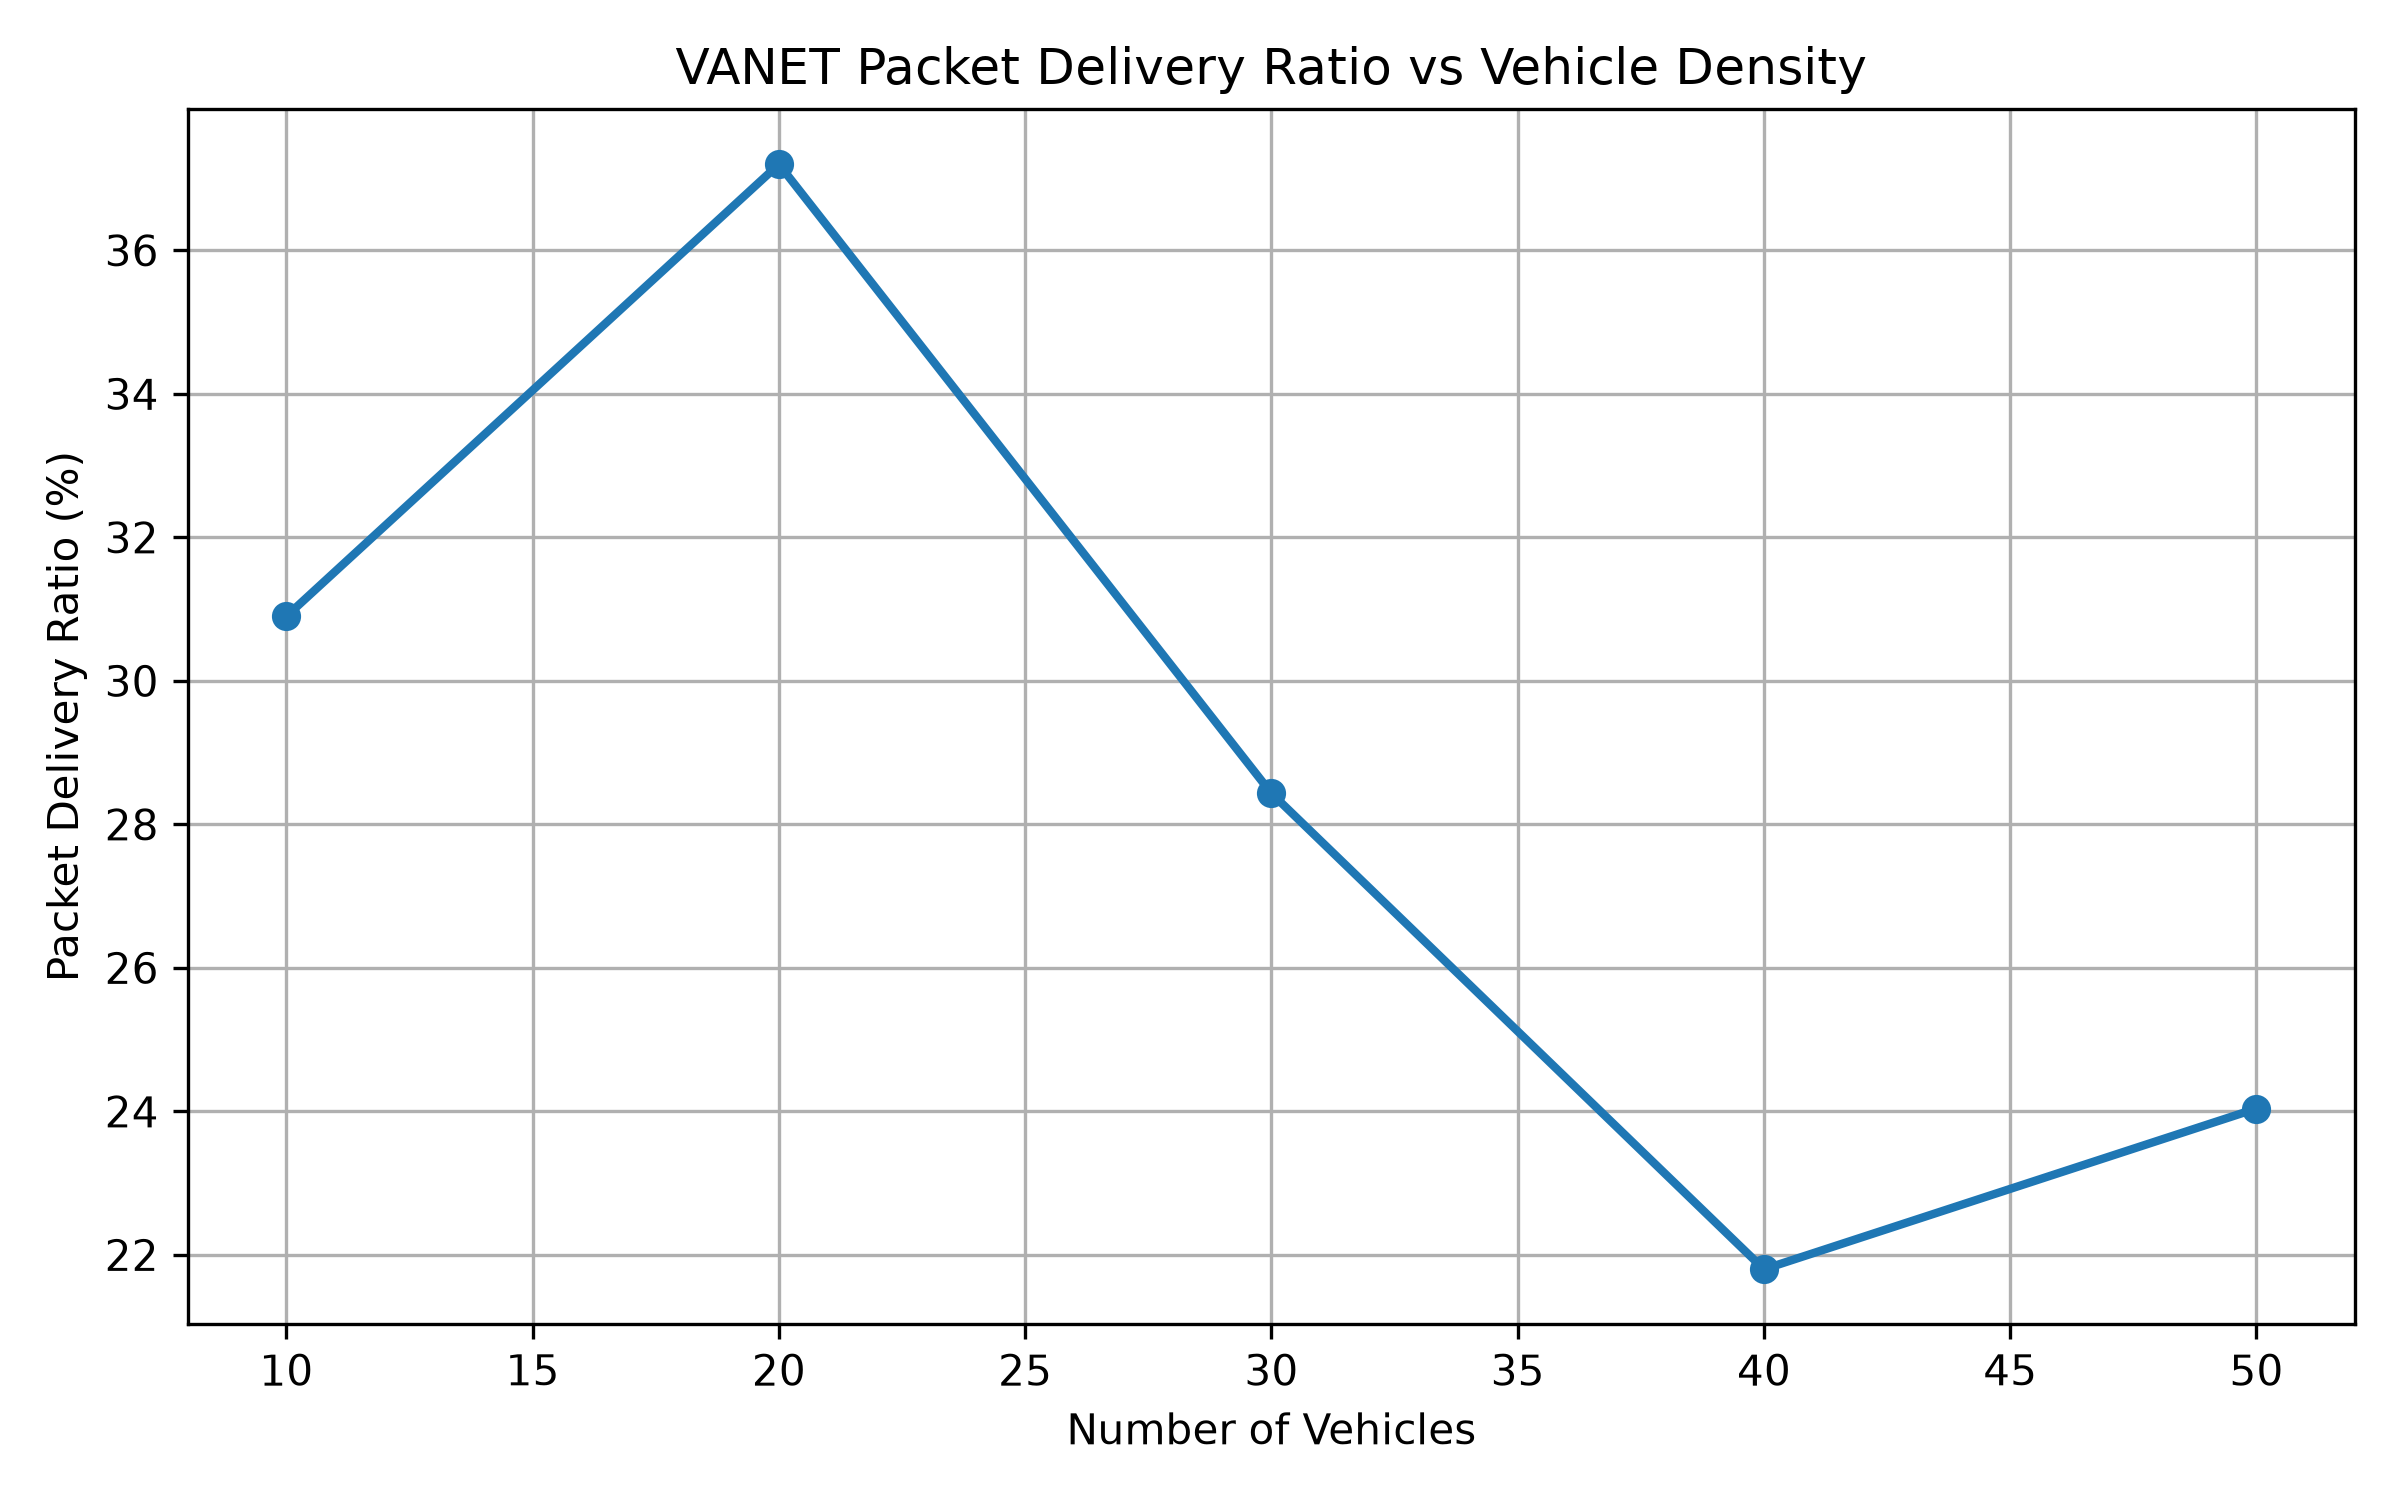
\includegraphics[width=\columnwidth]{Figures/vanet_pdr.png}
\caption{Packet delivery ratio for different
vehicle counts in the simplified model.}
\label{fig:python_pdr}
\end{figure}

\begin{figure}[htbp]
\centering
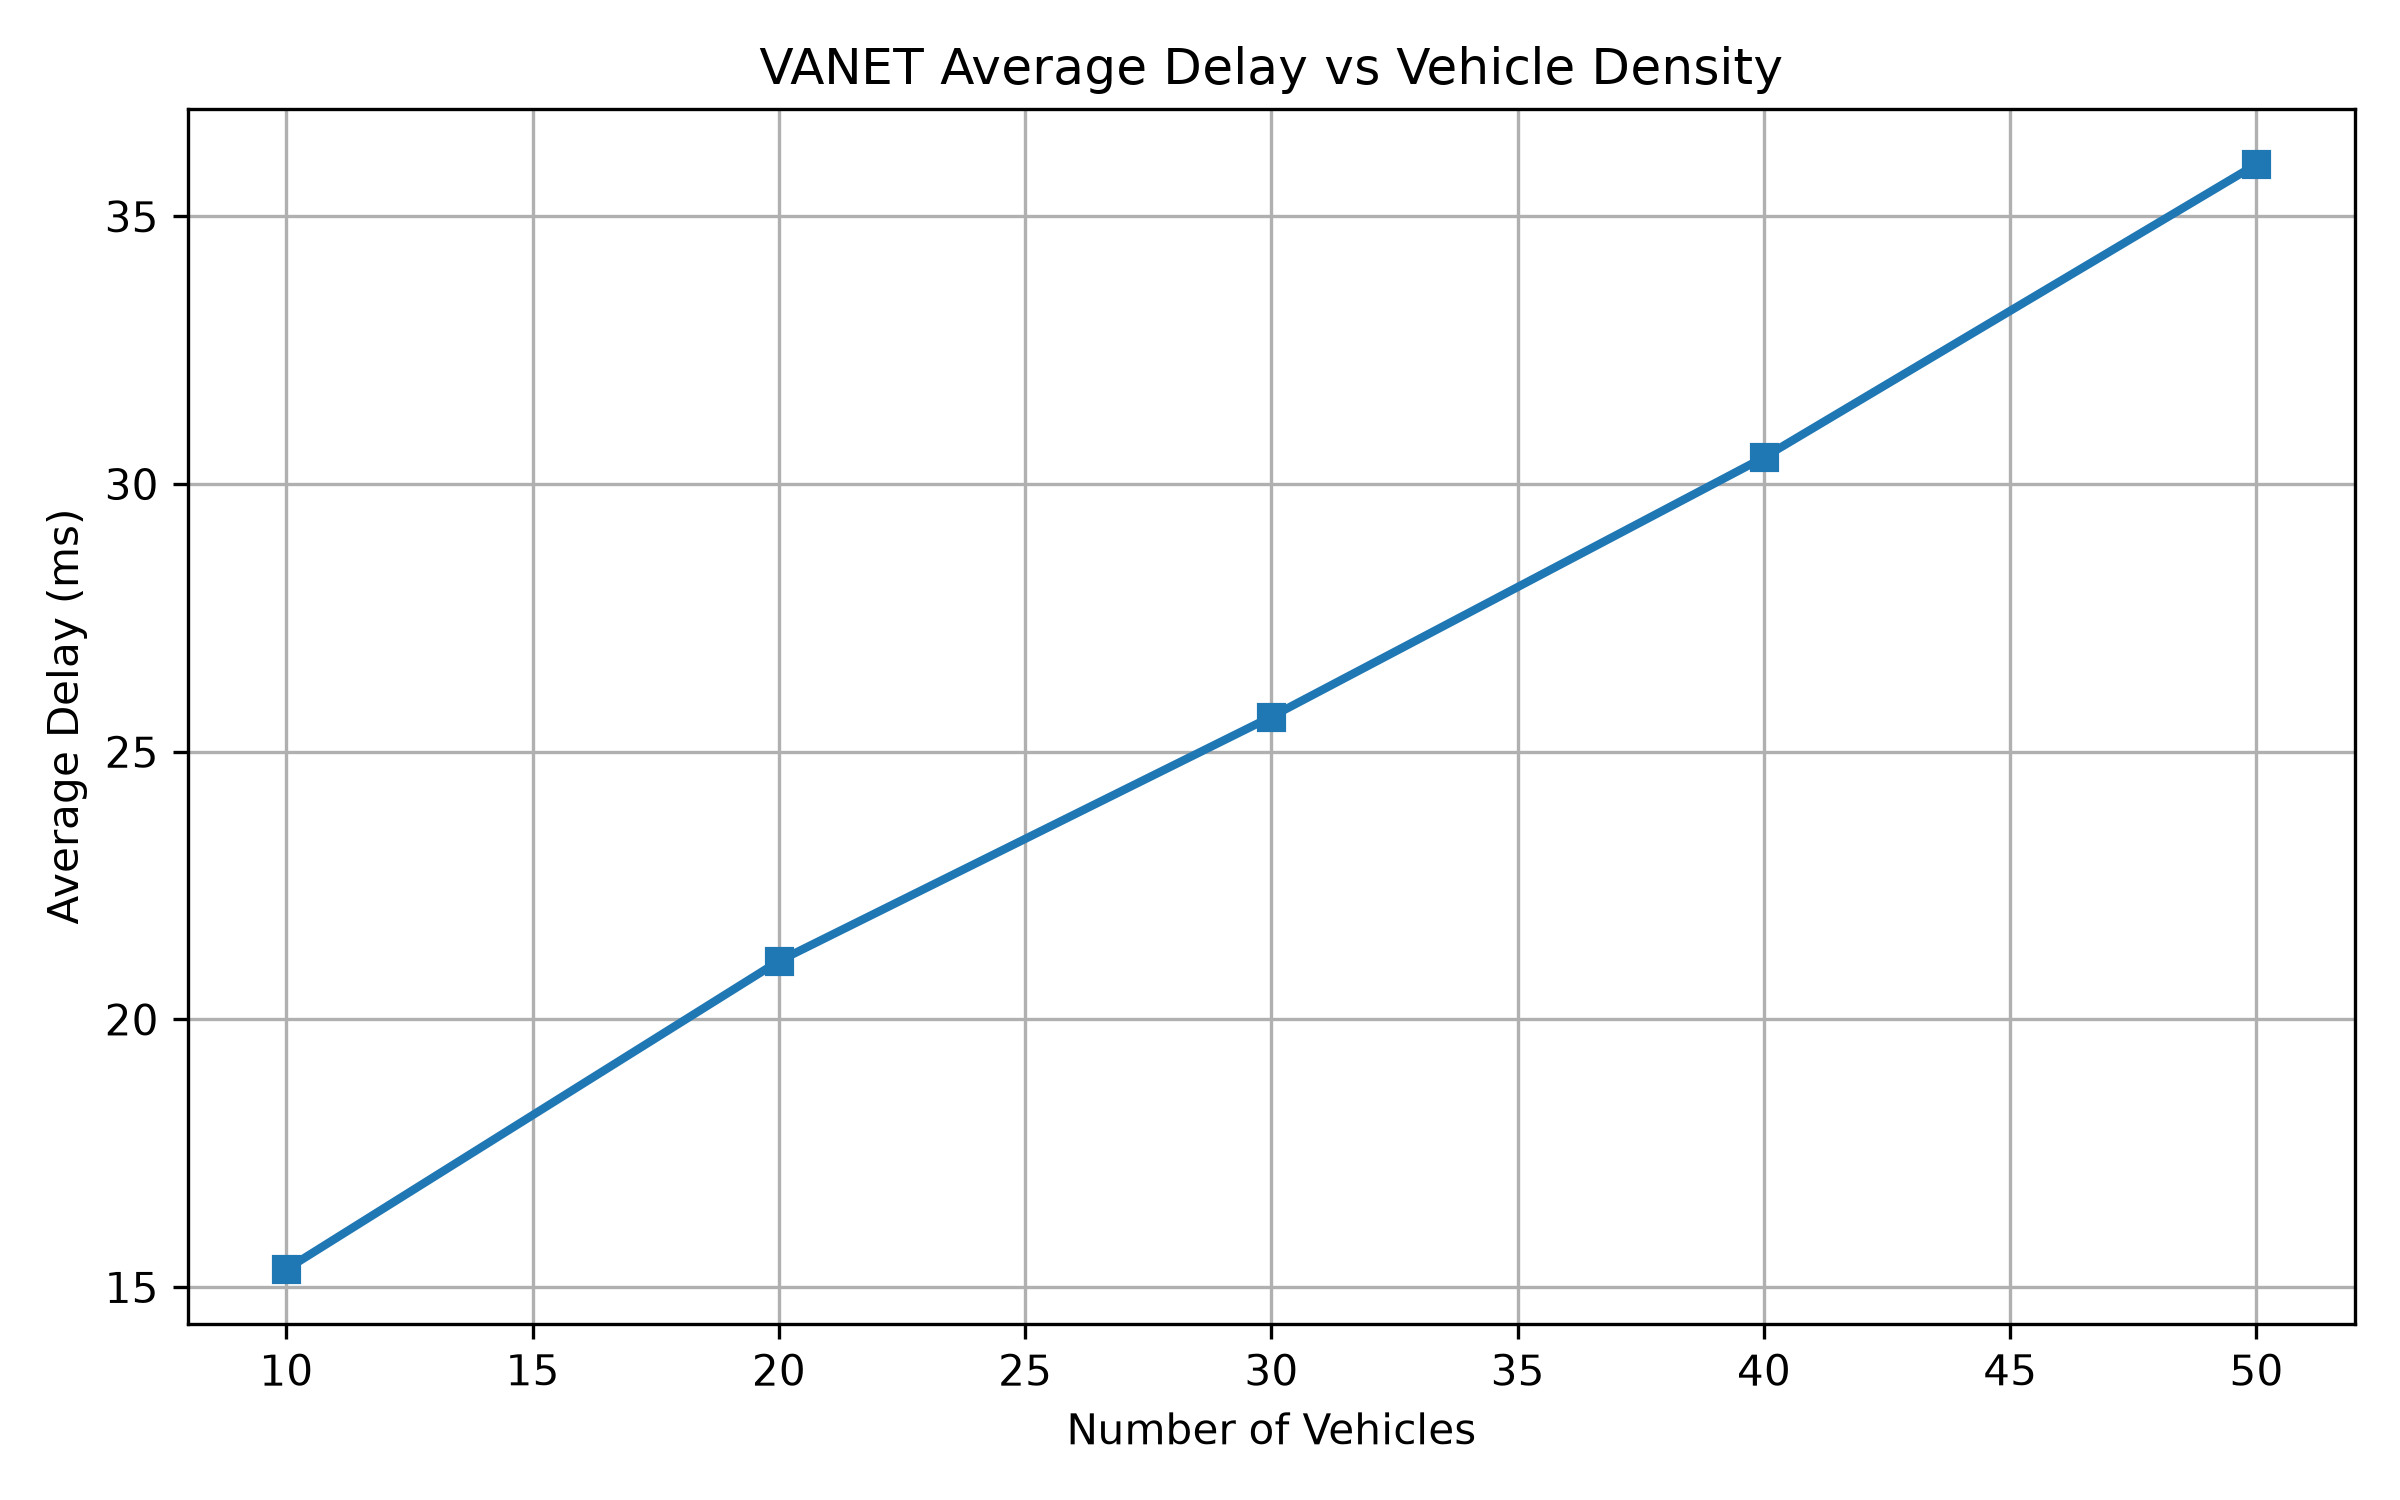
\includegraphics[width=\columnwidth]{Figures/vanet_delay.png}
\caption{Estimated average delay for different
vehicle counts in the simplified model.}
\label{fig:python_delay}
\end{figure}

\subsubsection{Results Discussion}

As shown in Fig.~\ref{fig:python_pdr},
the packet delivery ratio fluctuated
between 21.80\% and 37.20\%.

These variations reflect the random
vehicle positions, communication range,
and assumed packet success probabilities.

The results should not be interpreted
as measurements of an actual VANET
routing protocol.

Fig.~\ref{fig:python_delay} shows
that the estimated average delay
increased from 15.33 ms to 35.97 ms.

This increase is primarily explained
by the model's predefined delay formula,
which includes a term proportional
to the number of vehicles.

Therefore, the experiment demonstrates
the behavior of the selected mathematical
assumptions rather than independently
measuring real network congestion.

The experiment provides a reproducible
educational example of performance
evaluation concepts discussed in
the reviewed VANET literature.

\subsection{Discussion}
\label{sec:4H}

The reviewed frameworks demonstrate
that vehicular network evaluation
requires coordination between
mobility modeling and wireless
communication analysis.

SUMO provides detailed traffic
simulation, while OMNeT++ and
NS-3 provide network simulation
capabilities. Frameworks such
as Veins connect these
complementary components
to investigate communication
under changing traffic
conditions \cite{Sommer2011}.

The choice of simulation
environment should depend
on the research question
and required protocol models.

A study focused on vehicle
movement may emphasize
traffic simulation accuracy,
whereas a study focused on
wireless communication may
require detailed channel
and networking models.

Studies investigating
cooperative driving may
require both components
to exchange information
during execution.

Performance evaluation
must also reflect the
requirements of the
target application.

For example, packet delivery
ratio and delay are important
for safety-related communication,
while throughput and service
availability may be more relevant
to information-oriented services.

No single metric provides
a complete description
of VANET performance.

Furthermore, published results
must be interpreted in relation
to their experimental assumptions.
Differences in road topology,
vehicle density, wireless
technology, and traffic patterns
can produce different outcomes
even when the same routing
protocol is evaluated.

For these reasons, this paper combines
a review of established simulation
frameworks and performance metrics
with a simplified Python-based
illustrative experiment.

The numerical results reported in
Table~\ref{tab:python_results} and
Figs.~\ref{fig:python_pdr}--\ref{fig:python_delay}
are generated by the specified
probabilistic model. They demonstrate
selected evaluation concepts but do
not constitute validated measurements
of real-world VANET performance or
comparative tests of routing protocols.

A structured comparison of
published VANET studies can
help identify which approaches
are appropriate for particular
environments and where
important research gaps remain.
